\documentclass{article}

\usepackage{algorithmic}
\usepackage{amsmath}
\usepackage{graphicx}

\begin{document}

\title{Neural Network Handwriting Recognition}
\author{Geoffrey Ulman\\
        Midterm Exam\\
        CSI873}
\date{October 2011}
\maketitle

\tableofcontents

\section{Network Implementation}\label{Network Parameters}

The neural network used to classify the provided handwriting data set was a feed-forward network with 64 input nodes (one for each pixel in the input images), 10 output nodes (one for each digit 0 through 9), and one hidden layer. A number of different node counts for the hidden layer were tried and compared. The input and hidden layers also contained a threshold node whose output value was always fixed at \(1.0\). Each node in the hidden and output layers was implemented as a sigmoid threshold unit. Equation \ref{sigmoid1} demonstrates the calculations performed at a single node with inputs \(x_{0}\) through \(x_{n}\) and weights \(w_{0}\) through \(w_{n}\).


\begin{equation}\label{sigmoid1}
\begin{split}
net &= \sum\limits_{i=0}^n w_{i}x_{i}\\
\sigma_{net} &= \frac{1}{1+e^{-net}}
\end{split}
\end{equation}

\subsection{Name2}\label{Name2}

\begin{figure}
\centering
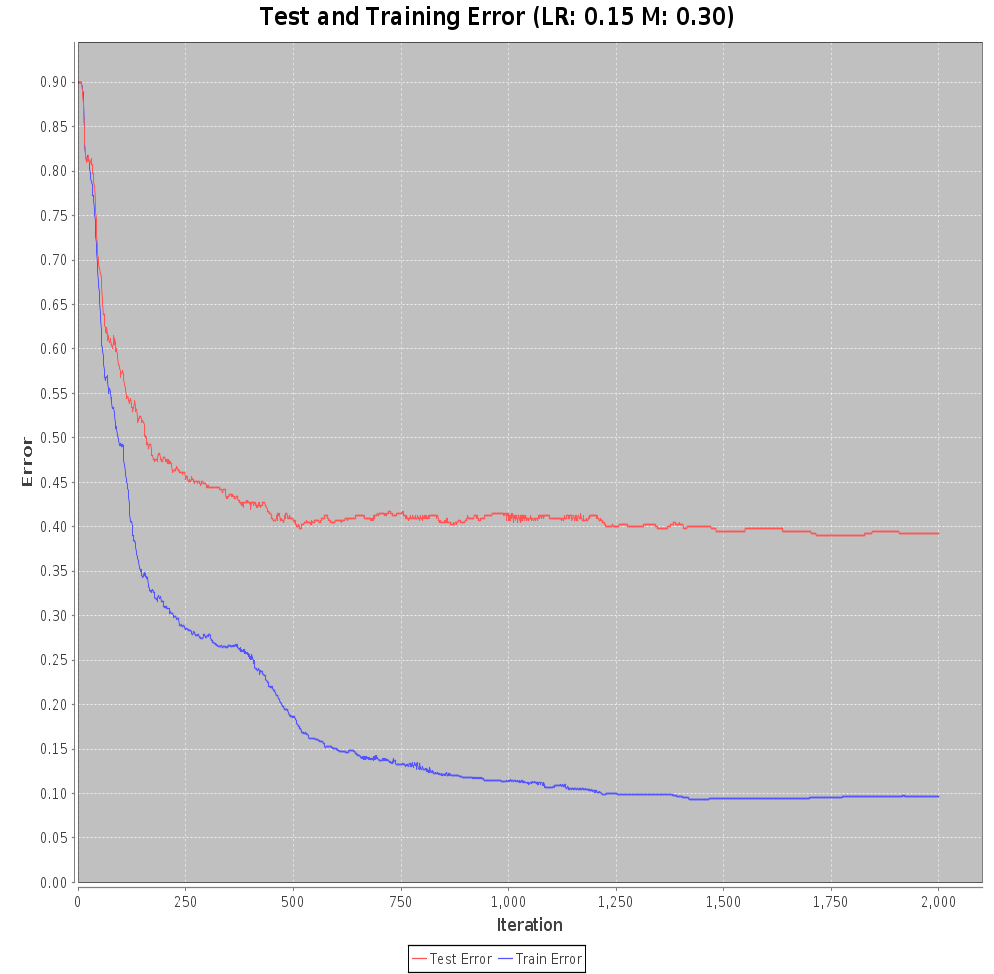
\includegraphics[width=0.85\textwidth]{data/0.15_0.3/64-10-10_15_3_error.png}
\caption{Prior Particle Position Distribution}
\label{prior}
\end{figure}

\begin{thebibliography}{9}

\bibitem{cpl}
  Brian W. Kernighan and Dennis M. Ritchie,
  \emph{The C Programming Language},
  Prentice Hall PTR, New Jersey,
  2009.

\bibitem{bmtt}
  Stone, Barlow, and Corwin,
  \emph{Bayesian Multiple Target Tracking},
  Artech House, Boston,
  1999.

\bibitem{oprc}
   Harris, Mark,
   \emph{Optimizing Parallel Reduction in CUDA},
   NVIDIA Developer Technology \\
   http://developer.download.nvidia.com/compute/cuda/sdk/website/samples.html

\bibitem{tutorial1}
   Volume I: Introduction to CUDA Programming \\
   http://www.nvidia.com/docs/IO/47904/VolumeI.pdf

\bibitem{bestprac}
   CUDA Best Practices Guide -- CUDA 2.2\\
   http://developer.download.nvidia.com/compute/cuda/2\_3/\\
   toolkit/docs/NVIDIA\_CUDA\_BestPracticesGuide\_2.3.pdf

\bibitem{thrust}
   Thrust C++ Template Library for CUDA \\
   http://code.google.com/p/thrust/

\bibitem{lcg}
   Linear Congruential Generator \\
   http://en.wikipedia.org/wiki/Linear\_congruential\_generator

\bibitem{pf}
   Particle Filter \\
   http://en.wikipedia.org/wiki/Particle\_filter

\end{thebibliography}

\end{document}
